\subsection{Counting 数数}
\begin{paracol}{2}
Counting is one of the basic skills when we learn numbers. And it is the basis of arithmetic. "Skip Counting" is counting by a number that is not 1. Learning to "Skip Count" helps you count many things quickly and learn your multiplication tables. 
 
\switchcolumn[1]
数数是我们在学习了数字以后所学习的,它是所有计算的基础。除了连续的数数,我们也应该学会跳着数数。它可以帮助我们数的更快,也是学习乘法口诀的基础。
\switchcolumn[0]*
For counting problems, you should be careful that miss anything and should not count something more than once. 
\switchcolumn[1]
对于数数的问题,最重要的就是不要漏掉,不应重复,如果漏掉了要加上,如果重复了要剪掉。
\end{paracol}

\begin{example}
How many line segments in the graph? 数一数下图中有多少条线段?
\begin{center}
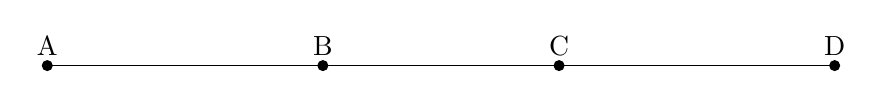
\begin{tikzpicture}[x=5cm,y=0.4cm]
    \draw (-1,0) coordinate (a) node[above] {A};
    \draw (-0.3,0) coordinate (b) node[above] {B};
    \draw (0.3,0) coordinate (c) node[above] {C};
    \draw (1,0) coordinate (d) node[above] {D};
     \fill (-1,0) circle[radius=2pt];
    \fill (-0.3,0) circle[radius=2pt];
     \fill (0.3,0) circle[radius=2pt];
     \fill (1,0) circle[radius=2pt];
    \path[draw] (a) -- (b) -- (c) -- (d);
\end{tikzpicture}
\end{center}
\end{example}
\begin{solution}
\begin{itemize}
\item Continuous points 连续两点:AB, BC, CD
\item Every other points 隔一个点:AC, BD
\item Every other two points 隔两点:AD
\end{itemize}
Therefore, there are 6 line segments. 因此,总共有6条线段。
\end{solution}

\begin{example}
Several people are in one row. There are 6 people in front of David and 8 people behind. How many people are there in this row? 一些人排成一列,在David的前面有6人,后面有8人,问这列队共有多少人?
\end{example}
\begin{solution}
As shown in the graph, 如图所示:
\begin{center}

\begin{tikzpicture}[x=5cm,y=0.4cm]
    \draw (0,0) coordinate (a) node[above] {David};
     \draw (-0.7,0) circle[radius=5pt];
     \draw (-0.6,0) circle[radius=5pt];
     \draw (-0.5,0) circle[radius=5pt];
     \draw (-0.4,0) circle[radius=5pt];
     \draw (-0.3,0) circle[radius=5pt];
     \draw (-0.2,0) circle[radius=5pt];
    \fill (0,0) circle[radius=5pt];
    \draw (0.2,0) circle[radius=5pt];
    \draw (0.3,0) circle[radius=5pt];
    \draw (0.4,0) circle[radius=5pt];
    \draw (0.5,0) circle[radius=5pt];
    \draw (0.6,0) circle[radius=5pt];
    \draw (0.7,0) circle[radius=5pt];
    \draw (0.8,0) circle[radius=5pt];
    \draw (0.9,0) circle[radius=5pt];
\end{tikzpicture}
\end{center}

There are 15 people in the line. 总人数是15人。
\end{solution}
\newpage